\chapter{User Interfaces}

\section{Introduction}
Android gives some key components that can be used to create user interface. All the Android user interface are built using these key components:

\begin{description}
	\item[View] It is the base class for all visual components (control and widgets). All the controls present in an android app are derived
	from this class. A View is an object that draws something on a smartphone screen and enables an user to interact with it.
	\item[Viewgroup] A ViewGroup can contain one or more Views and defines how these Views are placed in the user interface
	(these are used along with Android Layout managers.
	\item[Fragments] This component encapsulates a single piece of UI interface. They are very useful
	when we have to create and optimize our app user interface for multiple devices or multiple screen size.
	\item[Activities] Usually an Android app consists of several activities that exchange data and information. An Activity takes
	care of creating the user interface.
\end{description}

If we analyze in more detail an Android user interface, we can notice that it has an hierarchical structure where at the root there's
a ViewGroup. A ViewGroup behaves like an invisible container where single views are placed following some rules. We
can combine a ViewGroup with another ViewGroup to have more control on how views are located. We have to remember that complex user interfaces require more time to render it. 

\begin{framed}
Therefore, for better performance we should create
simple UIs.  Additionally, a clean interface helps user to have a better experience when using our app.	
\end{framed}


Before we continue we need to define some key concepts:

\begin{description}
	\item[Screen size] It is the physical screen or in other words, the real dimension of our device screen.
	\item[Density] It is the number of pixels in a given area. Usually we consider dot per inch (dpi). This is a measure of the screen
	quality.
	\item[Orientation] This is how the screen is oriented. It can be landscape or portrait.
	\item[Density independent pixel] This is a new pixel unit measure introduced by Android. It is called dp. One dp is equivalent at
	one pixel at a 160dpi screen. We should use dp unit in our measures when creating an UI, at the runtime the system takes care of
	converting it into a real pixel.
\end{description}

From the screen size point of view, Android groups the devices in four areas,small, normal, large and extra large (xlarge),
depending on the actual screen dimension expressed in inches. From the dpi point of view, on the other hand, we can group
devices in: ldpi (low dpi), mdpi (medium dpi), hdpi (high dpi), xhdpi (extra high dpi) and lately xxhdpi. This is important when
we use drawables (i.e bitmaps), because we have to create several images according to the different screen resolution.

There are some best practices regarding the user interface which we would already like to give:

\begin{framed}
	
	
	\begin{enumerate}
		\item Don’t use fixed dimensions expressed in pixel, instead we should use dp.
		\item Provide several layout structures for different screen size, we can do it creating several layout files.
		\item Provide several bitmap with different resolution for different screen resolutions. 
	\end{enumerate}

\end{framed}



\section{Understanding the View}
The View class is the basic class that all the components extend. A View draws something on a piece of screen and it is
responsible to handle events while user interacts with it. Even the generic ViewGroup class extends View. A ViewGroup
is a special View that holds other views and places these views following some rules.


All views have a set of properties: These properties affect the way the view is rendered. There is a set of properties common
to all views, while there are some other properties depending on the type of view.

\begin{description}
	\item[Focus] The system manages the focus on each view and depending on the user input, we can modify and force the focus on a
	specific view.
	\item[Listeners] All views have listeners which are used to handle events when the user interacts with the view. We can register our
	app to listen to specific events that occur on a view.
	\item[Visibility] We can control if a view is visible or not and we can change the view visibility at runtime too.
\end{description}
Two properties that play an important role are \texttt{layout\_width} and \texttt{layout\_height}. These two properties define how large
and how tall should be the view. We can use two predefined values:
\begin{itemize}
	\item \texttt{MATCH\_PARENT} we want our view as big as its parent that holds it
	\item \texttt{WRAP\_CONTENT} we
	specify that our view must be big enough to hold its content.
\end{itemize}
There is another option: using a numeric value. In this case, we specify the exact measure of our view. In this case, the best
practice suggests using dp unit measure so that our view can be adapted to different screen density.


\subsection{You should listen to your View}
Listeners are an important aspect when developing UIs in Android. Generally speaking, when an user interacts with our app
interface, the system “creates” some events. Each view that builds our interface is capable of generating events and providing the means to handle them.

In our Activity there is a method called \texttt{findViewById} that can be used to get the reference to a View defined in our user
interface. Once we have the reference, we can handle the user click:

\begin{android}
b.setOnClickListener(new View.OnClickListener() {
	@Override
	public void onClick(View v) {
		// here we handle the event
	}
});	
\end{android}

\section{Containers and Layoutmanagers}
There are different layout managers which will layout the view it includes. We will not cover them here in detail, but you get a complete overview by checking out the application \texttt{Containers} from \cite{murphymarkl.2017}.




\section{UI consistency}
One of the biggest efforts made by Google was to define a well defined set of rules that helps developers to create appealing user
interfaces. At the same time, these rules help users to navigate through every app in the same way. We call this\textbf{ UI consistency}.
Android, moreover, guarantees to the developers the required flexibility to customize the app look and feel and make it unique.
These rules are known as UI patterns. Patterns are proven solution approaches to well known problems. Thus, having a well
defined UI pattern catalog and knowing when and where apply them, we can create appealing apps that are not only full of
interesting features but they are enjoyable by users and easy to use.

\subsection{The landing activity}
The top level view is the ''landing`` area of our app, so we have to reserve to it a special attention, because this is the first
thing an user sees of our app. There are some specific patterns (see e.g. \cite{Google2017c}) that can be applied when designing this view depending on the type of information we want to show. Some of them are:

\begin{itemize}
	\item \textbf{Fixed tabs} : when we want to give to
	the user an overview of the different views present in our app, so that a user can switch easily between them to show different type of information. See an example here \cite{Tamada2013}
	
	\item \textbf{Spinner}: is used when we want to move directly to a specific view, this is the case of a calendar app when we can use spinner to
	go directly to a specific month.
	
	\begin{xml}
		<Spinner
		android:id="@+id/spinner"
		android:layout_width="fill_parent"
		android:layout_height="wrap_content" />
	\end{xml}
	
	
	\item \textbf{Navigation drawer}: This is a sliding menu, usually at the left side of the
	smartphone screen, that can be opened and closed by the user. This pattern can be used when we have a multiple top level view
	and we want to give to the user a fast access to one of them, or we want to give to the user the freedom to move to one low level
	view directly. For an example see  \cite{Google2017a}
\end{itemize}

\subsection{Detail View}
The detail view is a low level view where a user can interact with data directly. It is used to show data and edit them. In this
kind of view the layout plays an important role to make data well organized and structured. At this level, we can implement
an efficient navigation to improve usability of our app. In fact, we can use swipe view pattern so that user can move between
different detail views. Depending on the type of component we use to show detail information to the user, we can implement
some low level patterns that simplify the user interaction with our app.


\section{Screen and UI performance}
\subsection{Building Views}
For each view in you app, Android goes through three steps to render on the screen:
\begin{itemize}
	\item Measure 
	\item Layout
	\item Draw
\end{itemize}

The measuring starts at the top node and walks the render tree of the layout: measuring the dimensions of each view to be displayed on the screen. Each view will provide dimensions to the parent for positioning. If a parent view discovers an issue in the measurements of the dimensions (or that of its children), it can force every child to remeasure in order to resolve the issue (potentially tripling the measurement time). This is the reason a flat (less nested) view tree is valuable. The deeper the nodes for the tree, the more nested the measurement and the calculation times are lengthened.

See e.g. Instagram! \cite{Kieft2014}


To make sure you don't use to much nested views, you can make use of the Hierarchy Viewer (Component Tree in Android studio): it is a great tool to investigate the construction of your view XML. 

\subsection{Asset reduction}
With a flat design and the number of views reduced, you can reduce the number of objects used in each view. Reusing the objects can be a good strategy here.

\subsection{Overdrawing the screen}
When Android draws the screen, it draws the parent first and then the childer view on top of the parent views. This can result in entire views being drawn on the screen and then these views are entirely cover up by the subsequent views. This is a waist of processor time and should be avoided. 

You can test overdraw using the Debug GPU Overdraw tool in the developer options menu (see \cite{Google2017b}).

 
\newpage
\section{Exercise}

\begin{exercise}
	Pixel art is a form of digital art, created through the use of software, where images are edited on the pixel level. In this exercise you will have to create an application which is able to create such a pixel art drawing. 
	
	Let us have a look at the PixelArt website: \href{https://www.pixilart.com/draw}{PixelArt}. The basic idea of your application is that you make this into an Android application. The following requirements should definitely be fulfilled:
	\begin{enumerate}
		\item Fill in a pixel with a background color by tapping, or sliding over the pixels. There should be a possibility to choose the color for the background.
		\item An extra choice of drawing method: adding text in pixel format, or drawing a circle, or drawing a line or \dots It us up to you which kind of extra drawing technique you implement.
	\end{enumerate}
	Other extra feature will end up in extra credits for this application. 
	
	Off course copy pasting code from existing repositories will end up in a not so pleasant time during the examination.
	

\end{exercise}
	\begin{figure}[b]
		\centering
	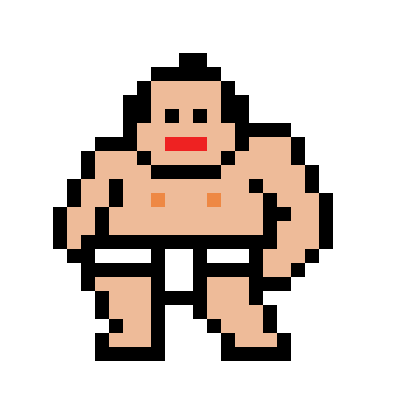
\includegraphics[width=0.4\textwidth]{images/ui/pixelart}
\end{figure}

